\chapter{Analyse et Conception}

\section{Modélisation}
Ce chapitre aborde la phase de conception du projet, une étape clé qui permet de transformer les besoins identifiés en une architecture technique claire et structurée. Nous y présentons nos choix méthodologiques, notamment l’usage du langage UML pour modéliser le système. Les diagrammes élaborés définissent le fonctionnement et l’organisation de l’application avant son implémentation. Cette démarche assure une base solide pour le développement et facilite la maintenance future du système.

\subsection{Choix méthodologique ?}
Dans le cadre de notre démarche méthodologique, parmis les differentes methodes de modelisation connus nous avons choisi d’utiliser le langage UML (Unified Modeling Language). Il permet de décrire les différents composants d’une application à travers des diagrammes clairs et organisés, facilitant ainsi la compréhension des besoins avant toute phase d’implémentation. L’un de ses principaux avantages réside dans son indépendance vis-à-vis des langages de programmation, ce qui permet de concevoir l’architecture logique du système sans contrainte technique immédiate.

\subsection{  UML}
L’UML (Unified Modeling Language) est un langage de modélisation graphique standardisé utilisé en génie logiciel pour analyser, concevoir et documenter un système informatique. Il repose sur l’approche orientée objet et permet de représenter de manière abstraite la structure et le comportement d’un logiciel avant son implémentation. UML propose un ensemble structuré de 14 diagrammes, regroupés en deux grandes catégories:\\ \\
Les diagrammes structurels ou diagrammes statiques qui sont au nombre de Sept (7), ils décrivent l’architecture statique du système, notamment les classes, les composants, les objets et leurs relations.
\begin{itemize}
\item Diagramme de classes;
\item Diagramme d’objets;
\item Diagramme de composants
\item Diagramme de déploiement;
\item Diagramme de paquetages;
\item Diagramme de structure composite;
\item Diagramme de profil.
\end{itemize} \\[5cm] \newline

Les diagrammes comportementaux ou diagrammes dynamiques qui sont au nombre de Sept (7), ils modélisent le fonctionnement dynamique du système, incluant les interactions, les processus, les cas d’utilisation et les séquences d’exécution.
\begin{itemize}
\item Diagramme de cas d'utilisation;
\item Diagramme d’activités;
\item Diagramme d'états;
\item Diagramme de séquence;
\item Diagramme de communication;
\item Diagramme de temps;
\item Diagramme global d’interaction.
\end{itemize}

Cette diversité de diagrammes permet d’analyser un système sous plusieurs angles complémentaires : organisation interne, interactions entre acteurs, flux d’activités, ou encore communication entre composants.

\section{Acteurs du système}

Dans notre application, l’acteur central est l’Utilisateur. Il désigne toute personne qui se connecte à la plateforme afin de consulter les informations météorologiques et d’exploiter les différentes fonctionnalités mises à disposition. En réalité, c’est autour de lui que le système a été conçu, puisque l’objectif principal de l’application est de rendre les données météorologiques accessibles, claires et personnalisables selon les besoins de chacun.

Toutefois, tous les utilisateurs ne disposent pas des mêmes droits. Afin d’organiser correctement les responsabilités, nous distinguons un profil particulier : l’Administrateur. Celui-ci constitue une spécialisation de l’Utilisateur. Autrement dit, il bénéficie de l’ensemble des fonctionnalités classiques, mais possède également des privilèges supplémentaires liés à la gestion et à la supervision du système.

De manière générale, l’Utilisateur peut :
\begin{enumerate}
    \item Consulter la météo en temps réel ;
    \item Visualiser les prévisions à court et moyen terme ;
    \item Rechercher la météo d’une ville spécifique ;
    \item Explorer des graphiques et des cartes interactives ;
    \item Personnaliser ses préférences (unités, langue, thème, notifications) ;
    \item Recevoir des alertes météorologiques.
\end{enumerate}

Pour réaliser ces actions, il interagit avec l’interface de l’application. Celle-ci communique ensuite avec le backend afin de récupérer les données stockées dans la base et de les afficher de manière claire et structurée.

De son côté, l’Administrateur occupe un rôle plus technique et organisationnel. En plus des fonctionnalités standards accessibles à tout utilisateur, il est responsable de :
\begin{enumerate}
    \item Gérer les stations météorologiques ;
    \item Superviser et contrôler les données reçues ;
    \item Assurer la maintenance et le bon fonctionnement du système ;
    \item Administrer les comptes utilisateurs.
\end{enumerate}

Ainsi, l’Administrateur contribue directement à la stabilité, à la sécurité et à la fiabilité globale de l’application. Dans le diagramme UML, cette distinction est représentée par une relation de généralisation, indiquant que l’Administrateur hérite des comportements de l’Utilisateur tout en disposant de responsabilités supplémentaires.

Enfin, on a la Station de base qui constitue l’acteur technique du système. Contrairement à l’Utilisateur et à l’Administrateur, elle n’interagit pas avec l’interface de l’application. Son rôle est différent : elle agit en amont du système en collectant les données météorologiques directement sur le terrain.

En effet, la station est équipée de plusieurs capteurs qui mesurent en continu différents paramètres environnementaux.Ces mesures sont collectees puis envoyées périodiquement vers la base de donnees Mongo. Parmi les informations transmises au système, on retrouve notamment :
\begin{enumerate}
    \item La température ;
    \item L’humidité ;
    \item La pression atmosphérique ;
    \item La vitesse du vent ;
    \item Les précipitations.
\end{enumerate} 

Ainsi, même si la Station de base ne participe pas directement à l’utilisation de l’interface, elle joue un rôle fondamental dans le fonctionnement global du système, puisqu’elle constitue la source principale des données exploitées par la plateforme.

\section{Diagrammes}
\subsection{Diagramme de contexte}
Le diagramme de contexte présente une vue globale du système URGmetEO et définit clairement ses frontières. Le système est représenté comme une entité unique qui interagit avec son environnement externe. Deux acteurs principaux apparaissent autour du système. D’une part, la Station de base, qui transmet les mesures météorologiques (température, humidité, pression, vent, précipitations) afin d’alimenter la plateforme. D’autre part, l’Utilisateur, qui consulte les informations fournies par le système, telles que la météo en temps réel, les prévisions et les visualisations graphiques. L’Administrateur est modélisé comme une spécialisation de l’Utilisateur, ce qui signifie qu’il hérite des mêmes interactions tout en disposant de droits supplémentaires liés à la gestion du système.
\begin{figure}[H]
\centering
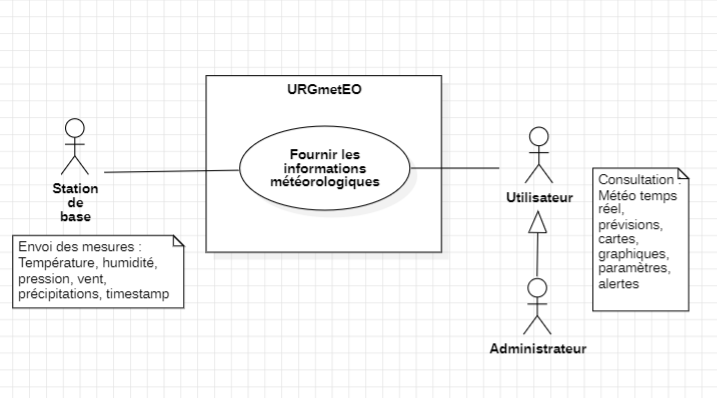
\includegraphics[width=0.7\textwidth]{Diagramme de contexte.png}
\caption{Diagramme de contexte du système}
\label{fig:diagramme_contexte}
\end{figure}

\subsection{Diagrammes des cas d’utilisation}
Les diagrammes de cas d’utilisation permettent de représenter, de manière simple, les services offerts par le système et la façon dont les différents acteurs interagissent avec lui. Ils constituent une étape importante de la modélisation, car ils traduisent les besoins fonctionnels identifiés lors de l’analyse.\\
Afin de mieux structurer cette partie, nous présentons un diagramme distinct pour chaque acteur. Cette séparation facilite la lecture et permet de comprendre plus clairement le rôle de chacun au sein du système.

\subsubsection{Diagramme de cas d’utilisation – Utilisateur}
Ce diagramme présente les différentes interactions possibles entre l’acteur \textbf{Utilisateur} et la plateforme URGmetEO. Il met en évidence les fonctionnalités qui permettent à un utilisateur de consulter et d’exploiter les informations météorologiques disponibles dans le système. Les principaux cas d’utilisation associés à cet acteur sont les suivants :

\begin{itemize}
    \item Consulter la météo en temps réel
    \item Consulter les prévisions météo
    \item Rechercher une ville
    \item Visualiser les graphiques météo
    \item Recevoir des alertes météo
    \item Configurer l’application
    \item S’authentifier
\end{itemize} \\

\noindent La fonctionnalité centrale du système est la consultation de la météo en temps réel. À partir de celle-ci, l’utilisateur peut effectuer certaines actions complémentaires telles que la recherche d’une ville, la visualisation des graphiques météorologiques ou la réception d’alertes. Ces fonctionnalités sont représentées dans le diagramme par des relations \texttt{<<extend>>}, indiquant qu’elles viennent enrichir la consultation des données sans être obligatoires.\\
Par ailleurs, la configuration de l’application nécessite que l’utilisateur soit préalablement identifié. Pour cette raison, le cas d’utilisation \textit{Configurer l’application} inclut le cas \textit{S’authentifier} à travers une relation \texttt{<<include>>}. Cette organisation permet de garantir que certaines opérations, notamment celles liées à la personnalisation des paramètres, soient accessibles uniquement aux utilisateurs authentifiés.
\begin{figure}[H]
    \centering
   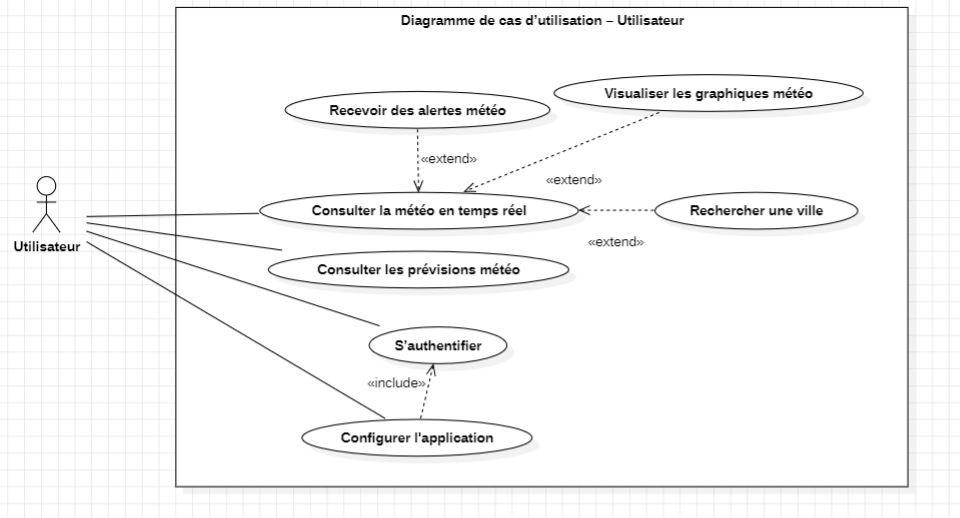
\includegraphics[width=0.7\textwidth]{Use case diagram Utilisateur.png}
    \caption{Diagramme de cas d’utilisation – Utilisateur}
    \label{fig:placeholder}
\end{figure}

\subsubsection{Diagramme de cas d’utilisation – Administrateur}

Ce diagramme illustre les différentes interactions entre l’acteur \textbf{Administrateur} et la plateforme URGmetEO. Contrairement à l’utilisateur classique, l’administrateur dispose de privilèges lui permettant de gérer les ressources du système, notamment les stations météorologiques et les comptes utilisateurs. Les principaux cas d’utilisation associés à cet acteur sont les suivants :

\begin{itemize}
    \item Ajouter une station
    \item Lister les stations
    \item Activer une station
    \item Désactiver une station
    \item Modifier une station
    \item Filtrer les données
    \item Lister les utilisateurs
    \item Activer un compte utilisateur
    \item Désactiver un compte utilisateur
    \item S’authentifier
\end{itemize}\\


\noindent Dans ce diagramme, la gestion des stations repose principalement sur le cas d’utilisation \textit{Lister les stations}. À partir de cette fonctionnalité, l’administrateur peut effectuer différentes actions telles que l’activation, la désactivation ou la modification d’une station. Ces opérations sont représentées par des relations \texttt{<<extend>>}, indiquant qu’elles viennent compléter la consultation de la liste des stations.\\

\noindent De la même manière, la gestion des utilisateurs s’effectue à partir du cas d’utilisation \textit{Lister les utilisateurs}. L’administrateur peut ensuite activer ou désactiver un compte selon les besoins de gestion du système.\noindent
Par ailleurs, plusieurs opérations incluent le cas d’utilisation \textit{S’authentifier}. Cette relation \texttt{<<include>>} indique que l’administrateur doit obligatoirement être identifié avant d’accéder aux fonctionnalités sensibles du système, notamment celles liées à la gestion des stations et des comptes utilisateurs.\\

\begin{figure}
    \centering
   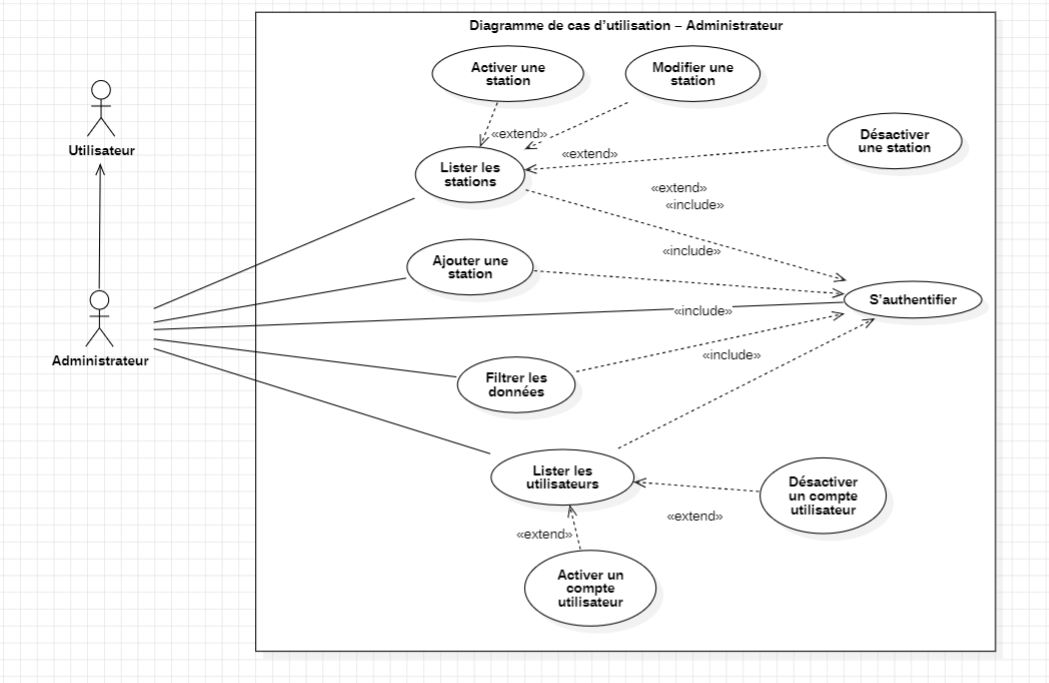
\includegraphics[width=0.7\textwidth]{Use case diagram Administrateur.png}
    \caption{Diagramme de cas d’utilisation – Administrateur}
    \label{fig:placeholder}
\end{figure}


\newpage
\subsubsection{Diagramme de cas d’utilisation – Station}

Ce diagramme présente les interactions entre l’acteur \textbf{Station de base} et la plateforme URGmetEO. Contrairement aux acteurs humains, la station de base est un dispositif technique chargé de fournir au système les données météorologiques collectées sur le terrain. Les cas d’utilisation associés à cet acteur sont les suivants :

\begin{itemize}
    \item Collecter les données météorologiques
    \item Transmettre les données météorologiques
\end{itemize}

\noindent La station est équipée de différents capteurs lui permettant de mesurer plusieurs paramètres environnementaux tels que la température, l’humidité, la pression atmosphérique, la vitesse du vent etc. Ces informations sont d’abord collectées par la station, puis transmises à la plateforme afin d’être enregistrées dans la base de données et exploitées par l’application.

\noindent Dans ce diagramme, le cas d’utilisation \textit{Transmettre les données météorologiques} inclut le cas \textit{Collecter les données météorologiques}. Cela signifie que la collecte constitue une étape préalable indispensable avant toute transmission des informations vers le système.
\begin{figure}
    \centering
    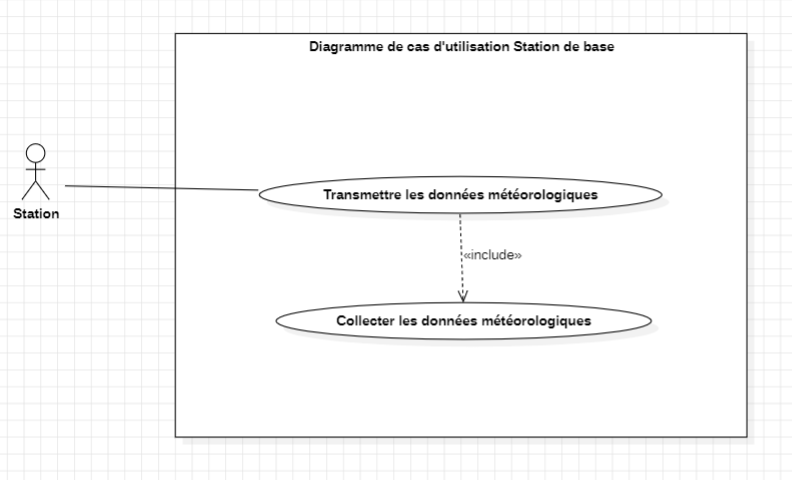
\includegraphics[width=0.7\textwidth]{Use case diagram Station.png} 
    \caption{Diagramme de cas d’utilisation – Station}
    \label{fig:placeholder}
\end{figure}








\subsection{Diagramme de classes}
Le diagramme de classes présente la structure statique de la plateforme URGmetEO à partir des modèles réellement implémentés. Il met en évidence les principales entités manipulées par l’application, leurs attributs, ainsi que les relations logiques déduites du modèle de données.
Les classes retenues sont :
\begin{itemize}
    \item \textbf{User} : gestion des comptes et informations d’authentification ;
    \item \textbf{authoritySchema} : gestion des rôles/autorités associés à un utilisateur ;
    \item \textbf{Station} : représentation des stations météorologiques (identité, localisation, état)
    \item \textbf{Device} : représentation d’un dispositif identifiant la source des mesures ;
    \item \textbf{Data} : enregistrement des mesures météorologiques (température, humidité, pression, etc.).
\end{itemize}

\noindent Du point de vue des relations entre les classes, un \textbf{User} peut être associé à plusieurs autorités (\textbf{authoritySchema}), ce qui permet de gérer les rôles et les droits d’accès des utilisateurs dans l’application. De plus, la classe \textbf{Device} est liée à la classe \textbf{Data}. En effet, un dispositif peut produire plusieurs enregistrements de données météorologiques. Chaque donnée est associée au dispositif qui l’a générée grâce à l’attribut \textit{deviceUUID}.
Enfin, dans l’implémentation actuelle, la classe \textbf{Station} ne possède pas de relation directe avec les autres classes du modèle. Elle apparaît donc comme une entité indépendante dans le diagramme.

\subsection{Diagramme d’activités}
\subsection{ Diagramme de séquence}


\section{Hiérarchie et architecture de l’application}

